% 23L-0723_NLP_Assignment-3.tex  --  compile with XeLaTeX (needed for Urdu script):
%   xelatex 23L-0723_NLP_Assignment-3.tex   (run 3 times for the table of contents)
% Figures in figures/ are produced by make_figures.py from ../results/results.json.
\documentclass[11pt,a4paper]{article}

\usepackage[margin=2.3cm,headheight=14pt]{geometry}
\usepackage{fontspec}
% Fonts are loaded by file name (Noto ships with TeX Live / MiKTeX), so no system install is needed.
\setmainfont{NotoSerif}[Extension=.ttf,UprightFont=*-Regular,BoldFont=*-Bold,ItalicFont=*-Italic,BoldItalicFont=*-BoldItalic,Scale=0.95]
\setsansfont{NotoSans}[Extension=.ttf,UprightFont=*-Regular,BoldFont=*-Bold,ItalicFont=*-Italic,BoldItalicFont=*-BoldItalic,Scale=0.95]
\setmonofont{NotoSansMono}[Extension=.ttf,UprightFont=*-Regular,BoldFont=*-Bold,Scale=0.85]
\usepackage{xcolor}
\usepackage{graphicx}
\usepackage{amsmath,amssymb}
\usepackage{booktabs,array,longtable,tabularx,multirow,colortbl}
\usepackage{listings}
\usepackage[most]{tcolorbox}
\usepackage{caption}
\usepackage{tikz}
\usetikzlibrary{positioning,arrows.meta,calc,fit,backgrounds}
\usepackage{pgfplots}
\pgfplotsset{compat=1.18}
\usepackage{microtype}
\usepackage{enumitem}
\usepackage{fancyhdr}
\usepackage{pifont}
\usepackage{float}

% ---------------- Semantic colour palette (data/statistics theme: analytical teal + one hot accent) ----------------
\definecolor{cData}{HTML}{2E7D6E}     % given data, inputs and outside knowledge (corpus, GloVe, "RNN + GloVe")
\definecolor{cModel}{HTML}{1F3A5F}    % model machinery: encoder/decoder blocks, the LSTM family
\definecolor{cBase}{HTML}{8A97A8}     % the baseline: plain (vanilla) RNN family
\definecolor{cKey}{HTML}{C8553D}      % THE thing to notice: best model (Transformer), attention, key findings
\definecolor{cNeutral}{HTML}{5B6472}  % structure: arrows, rules, captions, labels
\definecolor{cBg}{HTML}{F4F1EA}       % panel backgrounds
\colorlet{cDataL}{cData!10!white}
\colorlet{cModelL}{cModel!8!white}
\colorlet{cKeyL}{cKey!9!white}
\colorlet{cBaseL}{cBase!14!white}

\usepackage[colorlinks=true,linkcolor=cModel,urlcolor=cData,citecolor=cModel]{hyperref}

% Captions
\captionsetup{font=small,labelfont={bf,color=cNeutral},labelsep=period,margin=0.5cm}

% Headings in the model colour
\makeatletter
\renewcommand\section{\@startsection{section}{1}{\z@}{-3ex plus -1ex minus -.2ex}{1.5ex plus .2ex}{\normalfont\Large\sffamily\bfseries\color{cModel}}}
\renewcommand\subsection{\@startsection{subsection}{2}{\z@}{-2.5ex plus -1ex minus -.2ex}{1ex plus .2ex}{\normalfont\large\sffamily\bfseries\color{cModel}}}
\makeatother

% Header / footer
\pagestyle{fancy}\fancyhf{}
\fancyhead[L]{\small\sffamily\color{cNeutral}NLP Assignment 3: English $\rightarrow$ Urdu NMT}
\fancyhead[R]{\small\sffamily\color{cNeutral}\thepage}
\fancyfoot[L]{\footnotesize\sffamily\color{cNeutral}Mohammad Ibrahim Salman · 23L-0723}
\renewcommand{\headrulewidth}{0.4pt}\renewcommand{\headrule}{\color{cNeutral!50}\hrule height\headrulewidth}

% Boxes: one style per role
\newtcolorbox{defbox}[1][Key terms]{enhanced,breakable,colback=cModelL,colframe=cModel,boxrule=0.6pt,arc=2pt,
  fonttitle=\sffamily\bfseries\small,coltitle=white,title=#1,left=6pt,right=6pt,top=4pt,bottom=4pt}
\newtcolorbox{keybox}[1][Key finding]{enhanced,breakable,colback=cKeyL,colframe=cKey,boxrule=0.8pt,arc=2pt,
  fonttitle=\sffamily\bfseries\small,coltitle=white,title=#1,left=6pt,right=6pt,top=4pt,bottom=4pt}
\newtcolorbox{notebox}[1][Note]{enhanced,breakable,colback=cBg,colframe=cNeutral,boxrule=0.5pt,arc=2pt,
  fonttitle=\sffamily\bfseries\small,coltitle=white,title=#1,left=6pt,right=6pt,top=4pt,bottom=4pt}

% Code listings
\lstset{basicstyle=\ttfamily\small,backgroundcolor=\color{cBg},frame=single,rulecolor=\color{cNeutral!40},
  breaklines=true,columns=fullflexible,keepspaces=true,xleftmargin=4pt,xrightmargin=4pt,aboveskip=6pt,belowskip=6pt}

\linespread{1.1}% slightly more space between lines
\setlist{itemsep=2pt,topsep=3pt}
\newcommand{\term}[1]{\textbf{\textcolor{cModel}{#1}}}
\newcommand{\best}[1]{\textbf{\textcolor{cKey}{#1}}}
\newcommand{\ok}{\textcolor{cKey}{\ding{51}}}
\newcommand{\no}{\textcolor{cNeutral}{\ding{55}}}
\makeatletter\g@addto@macro\UrlBreaks{\do\_\do\-\do\.}\makeatother
\DeclareUrlCommand\file{\urlstyle{tt}}

% Urdu (right-to-left) support -- polyglossia loads bidi, so it comes last
\usepackage{polyglossia}
\setdefaultlanguage{english}
\setotherlanguage{urdu}
% Jameel Noori Nastaleeq (fonts/), the standard Urdu Nastaliq typeface. It has no bold, so bold is emboldened.
\newfontfamily\urdufont{JameelNooriNastaleeq.ttf}[Path=fonts/,Script=Arabic,Language=Urdu,Scale=1.25,AutoFakeBold=2]
\newfontfamily\urdufontsf{JameelNooriNastaleeq.ttf}[Path=fonts/,Script=Arabic,Language=Urdu,Scale=1.25,AutoFakeBold=2]
% Fixed height/depth so every Urdu row gets the same spacing (Nastaliq glyph heights vary a lot)
\newcommand{\ur}[1]{\mbox{\raisebox{0pt}[2.1ex][0.7ex]{\texturdu{#1}}}}

\begin{document}

% ---------------- Title block ----------------
\begin{titlepage}
\centering\setlength{\parindent}{0pt}
\vspace*{3.4cm}
{\fontsize{30}{36}\selectfont\bfseries\color{cModel} NLP Assignment 3\par}
\vspace{0.9cm}
{\Large English $\rightarrow$ Urdu Neural Machine Translation with\\[3pt]
RNN, BiRNN, LSTM, BiLSTM, Transformer and GloVe embeddings\par}
\vspace{1.1cm}
{\large\color{cNeutral} Natural Language Processing -- Course Assignment\par}

\vspace{2.0cm}
{\large
\begin{tabular}{@{}ll@{}}
\toprule
\textbf{Name} & \textbf{Roll number}\\
\midrule
Mohammad Ibrahim Salman & 23L-0723\\
\bottomrule
\end{tabular}\par}

\vfill
% Small emblem: an English token translated into an Urdu token
\begin{tikzpicture}[font=\small\sffamily]
  \node[rounded corners=4pt,draw=cModel,fill=cModel!12,thick,minimum width=1.3cm,minimum height=0.8cm] (en) at (0,0) {EN};
  \node[rounded corners=4pt,draw=cModel,fill=cModel,thick,text=white,minimum width=1.3cm,minimum height=0.8cm] (ur) at (2.6,0) {\large\texturdu{اردو}};
  \draw[-{Stealth[length=2.2mm]},thick,draw=cNeutral] (en) -- (ur);
\end{tikzpicture}\par
\vspace*{1.6cm}
\end{titlepage}

\tableofcontents
\vspace{0.6cm}
\begin{notebox}[How to read the colours in this document]
\begin{tabular}{@{}p{3.2cm}p{11.6cm}@{}}
\textcolor{cData}{\rule{8pt}{8pt}}\, \textbf{Teal} & data and outside knowledge: the corpus, the GloVe vectors, the ``RNN + GloVe'' model\\
\textcolor{cModel}{\rule{8pt}{8pt}}\, \textbf{Navy} & model machinery and the LSTM family\\
\textcolor{cBase}{\rule{8pt}{8pt}}\, \textbf{Slate} & the baseline: the plain RNN family\\
\textcolor{cKey}{\rule{8pt}{8pt}}\, \textbf{Vermilion} & the thing to notice: the best model (Transformer), attention, key findings\\
\textcolor{cNeutral}{\rule{8pt}{8pt}}\, \textbf{Grey} & structure: arrows, guides, labels\\
\end{tabular}

\smallskip
In plots, \emph{dashed} lines or hollow markers mean a \emph{bidirectional} encoder, so the figures still read in greyscale.
\end{notebox}

\newpage
% =====================================================================
\section{Setup}
% =====================================================================

The task is \term{machine translation}: a model reads an English sentence and writes the Urdu translation.
Every model here is an \term{encoder--decoder}. The \emph{encoder} reads the English sentence and turns it into numbers.
The \emph{decoder} uses those numbers to produce the Urdu sentence one word at a time.

\subsection{Dataset and preprocessing (Part 1)}

\textbf{Dataset:} \href{https://www.kaggle.com/datasets/zainuddin123/parallel-corpus-for-english-urdu-language}{Parallel corpus for English \& Urdu}
(Kaggle). It is a \term{parallel corpus}: two text files where line $i$ in one file is the translation of line $i$ in the other.
After removing empty lines there are \textbf{24,524 sentence pairs}. Most are short conversational sentences of 3--6 words.
Figure~\ref{fig:pipeline} shows the preprocessing steps.

\begin{figure}[htbp]
\centering
\begin{tikzpicture}[font=\small\sffamily,
  data/.style={rounded corners=6pt,draw=cData,fill=cDataL,thick,align=center,minimum height=1.25cm,text width=2.45cm},
  op/.style={draw=cModel,fill=cModelL,thick,align=center,minimum height=1.25cm,text width=2.45cm},
  arr/.style={-{Stealth[length=2.2mm]},thick,draw=cNeutral},
  node distance=0.55cm]
\node[data] (raw) {\textbf{2 text files}\\ english-corpus.txt\\ urdu-corpus.txt};
\node[op,right=of raw] (pd) {\textbf{1. Load}\\ Pandas DataFrame\\ 24,524 pairs};
\node[op,right=of pd] (tok) {\textbf{2. Tokenise}\\ split sentences\\ into words};
\node[op,right=of tok] (split) {\textbf{Split} 80/10/10\\ train / val / test\\ (seed 42)};
\node[op,below=1.0cm of split] (voc) {\textbf{Vocabulary}\\ from train only\\ cap 6,000 words};
\node[op,left=of voc] (pad) {\textbf{3. Pad}\\ every sequence\\ to 16 tokens};
\node[data,left=of pad] (ten) {\textbf{Tensors}\\ train 19,619 × 16\\ (same for all models)};
\draw[arr] (raw)--(pd); \draw[arr] (pd)--(tok); \draw[arr] (tok)--(split);
\draw[arr] (split)--(voc); \draw[arr] (voc)--(pad); \draw[arr] (pad)--(ten);
\end{tikzpicture}
\caption{Preprocessing turns two raw text files into fixed-size number grids that every model shares.
Rounded teal boxes are data; square navy boxes are operations. Steps 1--3 are the three Part~1 tasks.}
\label{fig:pipeline}
\end{figure}

\begin{enumerate}[label=\textbf{\arabic*.}]
\item \textbf{Load.} Both text files were loaded into a Pandas \emph{DataFrame} (a table with an \texttt{english} and an \texttt{urdu} column). Empty lines were dropped.
\item \textbf{Tokenise.} A \term{token} is one unit the model sees, here a word or a punctuation mark. \emph{Tokenising} means splitting a sentence into tokens.
  \begin{itemize}
  \item \textbf{English:} lower-cased word tokens, with punctuation split off.
  \item \textbf{Urdu:} Urdu punctuation (\ur{۔}\ \ \ur{؟}\ \ \ur{،}) is split off, then the text is split on whitespace.
  \end{itemize}
\item \textbf{Split} with a fixed seed into 80\% train (19,619 pairs), 10\% validation (2,452) and 10\% test (2,453).
  The \emph{validation} set is used to pick the best checkpoint. The \emph{test} set is only used for the final scores.
\item \textbf{Build vocabularies} from the training split only. A \term{vocabulary} is the list of known tokens; each gets an ID number.
  Both are capped at \textbf{6,000 tokens} and include the special tokens \texttt{<pad> <sos> <eos> <unk>}
  (padding, start of sentence, end of sentence, unknown word).
  The English vocabulary has 5,135 entries and the Urdu one has 5,134.
\item \textbf{Pad} every source and target sequence to \textbf{16 tokens}. \term{Padding} fills short sequences with \texttt{<pad>} so they all
  have the same length and can be stacked into one grid. Target sequences are wrapped in \texttt{<sos> \ldots\ <eos>}.
  This covers more than 99\% of sentences without truncation (cutting words off).
\end{enumerate}

The vocabulary and padding are shared by every model, as the assignment requires.

\subsection{Shared training configuration (identical for all models)}

Table~\ref{tab:config} lists the settings. Every model uses exactly these values, so differences in the results come from the architecture alone.

\begin{table}[htbp]
\centering\small
\caption{Shared training configuration. Every model uses these exact values.}
\label{tab:config}
\begin{tabularx}{\textwidth}{@{}l>{\raggedright\arraybackslash}p{4.6cm}>{\raggedright\arraybackslash}X@{}}
\toprule
\textbf{Setting} & \textbf{Value} & \textbf{What it means}\\
\midrule
Embedding dim & 200 (matches GloVe 6B-200d) & length of the vector that represents each word\\
Hidden size & 256 & size of the model's internal memory vector\\
Layers & 2 encoder + 2 decoder & how many processing layers are stacked\\
Dropout & 0.3 & randomly switch off 30\% of units while training\\
Optimiser & Adam, lr = 5e-4 & the rule for updating weights, and its step size\\
Batch size & 64 & sentence pairs processed per update\\
Epochs & \textbf{50} & full passes over the training data\\
Loss & cross-entropy, label smoothing 0.1, padding ignored & how wrong a prediction is\\
Gradient clipping & 1.0 & caps the size of each update\\
Decoding & greedy, max 16 tokens & how translations are produced at test time\\
Checkpoint & lowest validation loss & which saved weights are evaluated\\
Seed & 42 & fixes randomness so runs repeat exactly\\
\bottomrule
\end{tabularx}
\end{table}

\begin{defbox}[Key terms used in the configuration]
\begin{itemize}[leftmargin=12pt]
\item \term{Embedding}: a learned vector of numbers that stands for a word. Words used in similar ways end up with similar vectors.
\item \term{Epoch}: one full pass through all 19,619 training pairs.
\item \term{Dropout}: during training, randomly ignore some units so the model cannot rely on any single one. This reduces \emph{overfitting}.
\item \term{Overfitting}: the model memorises the training sentences instead of learning rules that work on new sentences.
\item \term{Cross-entropy loss}: a number that is low when the model gives high probability to the correct next word. Lower is better.
\item \term{Label smoothing (0.1)}: the training target gives 90\% to the correct word and spreads 10\% over the others, so the model does not become over-confident.
\item \term{Gradient clipping}: if an update would be larger than a limit (1.0), it is scaled down. This stops training from blowing up.
\item \term{Teacher forcing}: during training the decoder is fed the \emph{correct} previous Urdu word, not its own guess.
\item \term{Greedy decoding}: at test time, the decoder picks the single most likely word at each step until it outputs \texttt{<eos>}.
\end{itemize}
\end{defbox}

\subsection{Models (Part 2)}

Figure~\ref{fig:arch} contrasts the two kinds of architecture. The key difference is how much of the English sentence the decoder can see.

\begin{figure}[htbp]
\centering
\begin{tikzpicture}[font=\small\sffamily,
  cell/.style={draw=cModel,fill=cModelL,thick,minimum width=0.95cm,minimum height=0.75cm},
  tok/.style={rounded corners=4pt,draw=cData,fill=cDataL,thick,minimum width=0.95cm,minimum height=0.6cm},
  arr/.style={-{Stealth[length=1.8mm]},draw=cNeutral,thick}]
% --- Left: recurrent seq2seq ---
\node[font=\sffamily\bfseries\color{cModel}] at (3.0,3.6) {(a) Recurrent encoder--decoder};
\foreach \i/\w in {0/he,1/raised,2/his,3/hand}{
  \node[tok] (x\i) at (\i*1.15,0) {\w};
  \node[cell] (h\i) at (\i*1.15,1.25) {};
  \draw[arr] (x\i)--(h\i);
}
\foreach \i [evaluate=\i as \j using int(\i+1)] in {0,1,2}{ \draw[arr] (h\i)--(h\j); }
\node[draw=cNeutral,fill=cBg,very thick,circle,minimum size=0.9cm,font=\sffamily\bfseries\small] (c) at (1.72,2.55) {$c$};
\draw[arr] (h3) to[bend right=20] (c);
\node[align=right,anchor=east,font=\scriptsize\sffamily\color{cNeutral}] at (1.15,2.55) {one fixed 256-d\\vector (bottleneck)};
\foreach \i in {0,1,2}{
  \node[cell] (d\i) at (5.0+\i*1.15,1.25) {};
  \node[tok,draw=cModel,fill=white] (y\i) at (5.0+\i*1.15,0) {$y_{\i}$};
  \draw[arr] (d\i)--(y\i);
}
\draw[arr] (d0)--(d1); \draw[arr] (d1)--(d2);
\draw[arr,dashed] (c) to[bend left=15] (d0); \draw[arr,dashed] (c) to[bend left=10] (d1); \draw[arr,dashed] (c) to[bend left=8] (d2);
\node[font=\scriptsize\sffamily\color{cNeutral}] at (1.72,-0.7) {encoder (RNN or LSTM)};
\node[font=\scriptsize\sffamily\color{cNeutral}] at (6.15,-0.7) {decoder (Urdu words)};
% --- Right: Transformer ---
\begin{scope}[xshift=9.35cm]
\node[font=\sffamily\bfseries\color{cKey}] at (1.72,3.6) {(b) Transformer};
\foreach \i/\w in {0/he,1/raised,2/his,3/hand}{
  \node[tok] (tx\i) at (\i*1.15,0) {\w};
  \node[cell] (e\i) at (\i*1.15,1.25) {$e_{\i}$};
  \draw[arr] (tx\i)--(e\i);
}
\node[cell,draw=cKey,fill=cKeyL] (yt) at (1.72,2.65) {$y_t$};
\foreach \i in {0,1,2,3}{ \draw[-{Stealth[length=1.6mm]},draw=cKey,thick] (e\i)--(yt); }
\node[align=left,anchor=west,font=\scriptsize\sffamily\color{cKey}] at (2.35,2.65) {attention: looks\\at every English\\word};
\node[font=\scriptsize\sffamily\color{cNeutral}] at (1.72,-0.7) {encoder outputs, one per word};
\end{scope}
\end{tikzpicture}
\caption{(a) The recurrent models squeeze the whole English sentence into \emph{one} vector $c$, which every decoder step must reuse.
(b) The Transformer's decoder uses \textcolor{cKey}{attention} to look directly at every English word at every step, so nothing has to pass through a bottleneck.
This is a schematic, not real model values.}
\label{fig:arch}
\end{figure}

\begin{itemize}
\item \textbf{RNN / LSTM:} a sequence-to-sequence (\emph{seq2seq}) encoder--decoder in the style of Cho et al.\ (2014).
  \begin{itemize}
  \item An \term{RNN} (recurrent neural network) reads words one at a time and updates a memory vector after each word.
  \item An \term{LSTM} (long short-term memory) is an RNN with \emph{gates}: small learned switches that decide what to keep, forget and output. This lets it remember information over longer spans.
  \item The encoder is a 2-layer Elman RNN or LSTM. Sequences are \emph{packed} so padding is ignored.
  \item The final state initialises the decoder.
  \item The top-layer context vector is also fed to the decoder at every step and to the output layer.
  \item These models have no attention.
  \end{itemize}
\item \textbf{BiRNN / BiLSTM:} the same as above, but with a \term{bidirectional} encoder. It reads the sentence both left-to-right and right-to-left.
  The forward and backward final states of each layer are concatenated (joined end to end) and projected with Linear + tanh to the decoder's hidden size.
\item \textbf{Transformer:} \texttt{nn.Transformer} with 2 encoder and 2 decoder blocks, 8 attention heads, $d_\text{model} = 200$ and a feed-forward size of 512.
  \begin{itemize}
  \item \term{Attention} lets each output word compute a weighted mix of all encoder outputs, focusing on the most relevant English words.
  \item \term{Multi-head attention} runs 8 of these in parallel, so different heads can focus on different things (for example word order vs.\ word meaning).
  \item It uses sinusoidal \emph{positional encodings} (fixed sine/cosine patterns that tell the model each word's position), padding masks and a \emph{causal} decoder mask (the decoder cannot peek at future words).
  \end{itemize}
\item \textbf{RNN + GloVe:} the same RNN, but the English embedding layer starts from \texttt{glove.6B.200d} vectors and is then fine-tuned (allowed to keep changing during training).
  GloVe covers \textbf{98.2\%} of the English vocabulary (5,037 of 5,131 words).
\end{itemize}

% =====================================================================
\section{Results on the held-out test set (Part 3)}
% =====================================================================

All models were evaluated on the same \textbf{2,453 test sentences}, which no model saw during training.

\subsection{The metrics}

All scores are on a 0--100 scale; higher is better.
\begin{defbox}[Evaluation metrics]
\begin{itemize}[leftmargin=12pt]
\item \term{BLEU-4}: counts how many 1-, 2-, 3- and 4-word sequences (\emph{n-grams}) in the model's output also appear in the reference translation.
  It is computed over the whole test set (corpus-level). BLEU-1 counts single words only.
\[
\text{BLEU} = \text{BP}\cdot \exp\Big(\textstyle\sum_{n=1}^{4} \tfrac14 \log p_n\Big)
\]
  In words: $p_n$ is the fraction of the output's $n$-grams that match the reference, the four are averaged (geometrically), and BP is a \emph{brevity penalty} that lowers the score if outputs are too short.
\item \term{ROUGE-1 / ROUGE-2 / ROUGE-L}: F1 overlap between output and reference, using single words, word pairs, and the \emph{longest common subsequence} (the longest run of words appearing in the same order in both), averaged over sentences.
\item \term{METEOR}: matches words between output and reference, balances precision and recall, and penalises outputs where matched words are scattered (fragmentation). Averaged over sentences.
\item \term{chrF}: an F-score over character sequences (1--6 characters). It gives partial credit for nearly-right word forms.
\end{itemize}
\end{defbox}

\begin{notebox}[Notes on the metrics]
\begin{itemize}[leftmargin=12pt]
\item \textbf{ROUGE} is computed in the notebook on Urdu word tokens. The common \texttt{rouge\_score} package's default tokenizer drops non-Latin characters, so it would score every Urdu sentence as 0.
\item \textbf{METEOR} uses exact and stem matches only, because there is no Urdu WordNet (WordNet is an English synonym dictionary).
\item \textbf{chrF} is a character-level check that does not depend on how words are tokenised.
\end{itemize}
\end{notebox}

\subsection{Final scores}

Table~\ref{tab:scores} gives every score; Figure~\ref{fig:scores} shows the four main metrics side by side.

\begin{table}[htbp]
\centering\small
\caption{Test-set scores (0--100, higher is better). The \textcolor{cKey}{Transformer} is best on every metric.}
\label{tab:scores}
\begin{tabular}{@{}l *{7}{r}@{}}
\toprule
\textbf{Model} & \textbf{BLEU-4} & BLEU-1 & \textbf{ROUGE-1} & ROUGE-2 & \textbf{ROUGE-L} & \textbf{METEOR} & chrF\\
\midrule
\textcolor{cBase}{\textbf{RNN}}         & 32.76 & 59.74 & 60.93 & 38.82 & 60.59 & 52.71 & 49.04\\
\textcolor{cBase}{\textbf{BiRNN}}       & 33.07 & 59.73 & 61.14 & 39.44 & 60.77 & 52.81 & 49.33\\
\textcolor{cModel}{\textbf{LSTM}}       & 37.78 & 64.40 & 64.92 & 43.80 & 64.42 & 57.52 & 54.04\\
\textcolor{cModel}{\textbf{BiLSTM}}     & 37.22 & 63.95 & 64.45 & 42.99 & 64.07 & 56.77 & 53.00\\
\rowcolor{cKeyL}
\textcolor{cKey}{\textbf{Transformer}}  & \best{39.70} & \best{65.08} & \best{65.75} & \best{45.54} & \best{65.12} & \best{58.80} & \best{56.99}\\
\textcolor{cData}{\textbf{RNN + GloVe}} & 35.32 & 62.28 & 63.19 & 41.16 & 62.79 & 55.31 & 51.24\\
\bottomrule
\end{tabular}

\vspace{0.6cm}
\caption{Model size, best validation loss and training cost (50 epochs on a Tesla T4).
The Transformer is the smallest model (4.88\,M parameters) but the slowest per epoch (5.8\,s).}
\label{tab:cost}
\begin{tabular}{@{}l rrrrr@{}}
\toprule
\textbf{Model} & \textbf{Best val loss} & \textbf{Best epoch} & \textbf{Params} & \textbf{Train time (50 ep)} & \textbf{s / epoch}\\
\midrule
\textcolor{cBase}{\textbf{RNN}}         & 2.885 & 48 & 5.25 M & 162 s & 3.2\\
\textcolor{cBase}{\textbf{BiRNN}}       & 2.882 & 49 & 5.76 M & 177 s & 3.5\\
\textcolor{cModel}{\textbf{LSTM}}       & \textbf{2.747} & 48 & 6.94 M & 212 s & 4.2\\
\textcolor{cModel}{\textbf{BiLSTM}}     & 2.790 & 29 & 8.72 M & 246 s & 4.9\\
\textcolor{cKey}{\textbf{Transformer}}  & 2.824 & 50 & 4.88 M & 289 s & 5.8\\
\textcolor{cData}{\textbf{RNN + GloVe}} & 2.785 & 48 & 5.25 M & 161 s & 3.2\\
\bottomrule
\end{tabular}
\end{table}

Table~\ref{tab:cost} shows that the \textbf{LSTM} has the lowest validation loss, yet the Transformer translates best.
Loss measures how confidently the model predicts each next word \emph{when given the correct previous words};
the test scores measure the full translations the model writes on its own. The two do not have to agree exactly.

\begin{figure}[htbp]
\centering
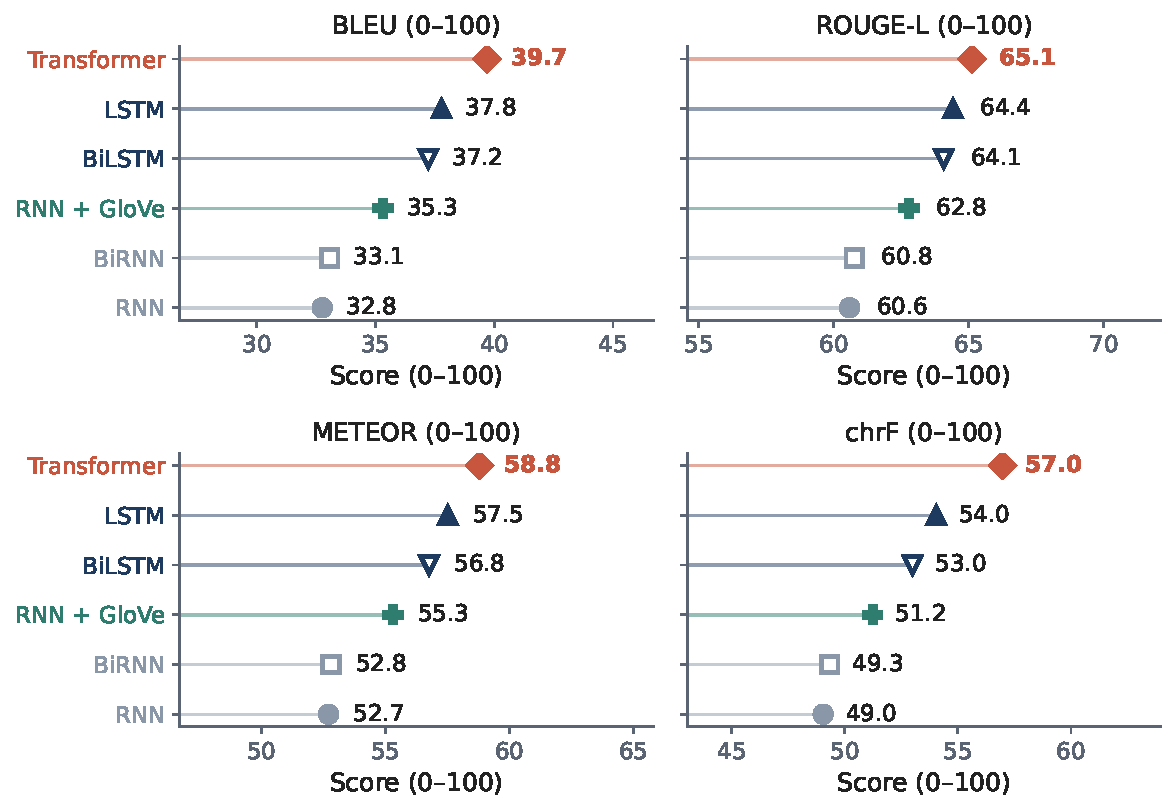
\includegraphics[width=0.85\textwidth]{figures/scores.pdf}
\caption{The \textcolor{cKey}{Transformer} (vermilion diamond) leads on all four metrics.
LSTMs (navy) beat plain RNNs (slate) by about 5 points, and GloVe (teal) lifts the RNN about halfway to the LSTMs. Hollow markers are bidirectional encoders.}
\label{fig:scores}
\end{figure}

Figure~\ref{fig:valloss} shows the validation loss for each model across all 50 epochs.

\begin{figure}[H]
\centering
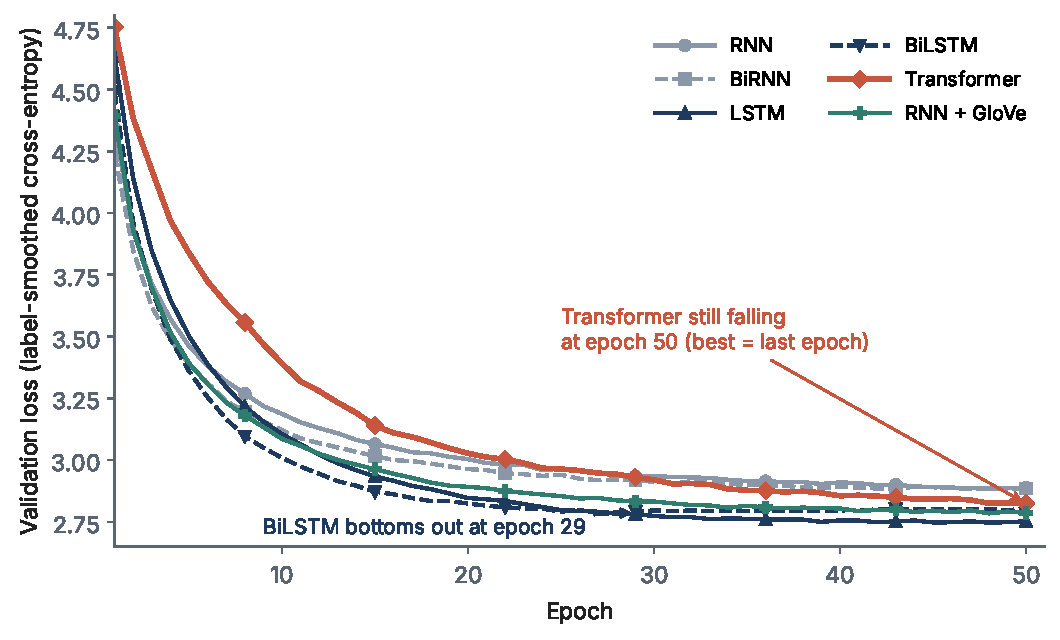
\includegraphics[width=0.85\textwidth]{figures/val_loss.pdf}
\caption{Validation loss per epoch. The recurrent models flatten out well before epoch 50, but the
\textcolor{cKey}{Transformer} is still improving at the end. Its best checkpoint is the last epoch, so it had not finished learning.}
\label{fig:valloss}
\end{figure}



\subsection{Inference examples}

Table~\ref{tab:examples} shows five of the 15 fixed test sentences. The other ten are in Appendix~\ref{app:examples}.
\ok\ marks an output identical to the reference, ignoring spacing and final punctuation.
Urdu is written right to left.

\begin{center}\small
\begin{longtable}{@{}p{2.6cm}>{\raggedleft\arraybackslash}p{10.6cm}c@{}}
\caption{Five fixed test sentences translated by every model. The \textcolor{cKey}{Transformer} matches the reference on 4 of the 5; no other model matches more than 2.}\label{tab:examples}\\
\toprule
\textbf{Model} & \textbf{Urdu output} & \textbf{=\,ref}\\ \midrule \endfirsthead
\toprule \textbf{Model} & \textbf{Urdu output} & \textbf{=\,ref}\\ \midrule \endhead
\bottomrule \endfoot
\rowcolor{cBg}\multicolumn{3}{@{}l@{}}{\textbf{EN:} \textit{he is an italian} \quad \textcolor{cNeutral}{Reference:} \ur{وہ ایک اطالوی ہے}}\\*
\textcolor{cBase}{\textbf{RNN}} & \ur{وہ ایک \textenglish{excon} ہے} & \\*
\textcolor{cBase}{\textbf{BiRNN}} & \ur{وہ ایک انگریز ہے} & \\*
\textcolor{cModel}{\textbf{LSTM}} & \ur{وہ ایک ماہر ہے} & \\*
\textcolor{cModel}{\textbf{BiLSTM}} & \ur{وہ ایک ماہر ہے} & \\*
\textcolor{cKey}{\textbf{Transformer}} & \ur{وہ ایک اطالوی ہے} & \ok\\*
\textcolor{cData}{\textbf{RNN + GloVe}} & \ur{وہ ایک فرانسیسی ہے} & \\
\addlinespace[3pt]
\rowcolor{cBg}\multicolumn{3}{@{}l@{}}{\textbf{EN:} \textit{zain is seldom home} \quad \textcolor{cNeutral}{Reference:} \ur{زین شاذ و نادر ہی گھر ہوتا ہے۔}}\\*
\textcolor{cBase}{\textbf{RNN}} & \ur{زین گھر گھر ہے} & \\*
\textcolor{cBase}{\textbf{BiRNN}} & \ur{زین گھر سے گھر ہے ۔} & \\*
\textcolor{cModel}{\textbf{LSTM}} & \ur{زین گھر سے گھر ہے ۔} & \\*
\textcolor{cModel}{\textbf{BiLSTM}} & \ur{زین گھر سے گھر ہے ۔} & \\*
\textcolor{cKey}{\textbf{Transformer}} & \ur{زین شاذ و نادر ہی گھر ہے ۔} & \\*
\textcolor{cData}{\textbf{RNN + GloVe}} & \ur{زین گھر سے گھر ہے ۔} & \\
\addlinespace[3pt]
\rowcolor{cBg}\multicolumn{3}{@{}l@{}}{\textbf{EN:} \textit{i need a new bicycle} \quad \textcolor{cNeutral}{Reference:} \ur{مجھے ایک نئی سائیکل چاہیے}}\\*
\textcolor{cBase}{\textbf{RNN}} & \ur{مجھے ایک نئی سائیکل چاہیے} & \ok\\*
\textcolor{cBase}{\textbf{BiRNN}} & \ur{مجھے ایک نئی سائیکل چاہیے} & \ok\\*
\textcolor{cModel}{\textbf{LSTM}} & \ur{میں ایک نئی سائیکل کی ضرورت ہے} & \\*
\textcolor{cModel}{\textbf{BiLSTM}} & \ur{میں ایک نئی الماری کی ضرورت ہے} & \\*
\textcolor{cKey}{\textbf{Transformer}} & \ur{مجھے ایک نئی سائیکل چاہیے} & \ok\\*
\textcolor{cData}{\textbf{RNN + GloVe}} & \ur{مجھے ایک نئی سائیکل چاہیے} & \ok\\
\addlinespace[3pt]
\rowcolor{cBg}\multicolumn{3}{@{}l@{}}{\textbf{EN:} \textit{i can sleep anywhere} \quad \textcolor{cNeutral}{Reference:} \ur{میں کہیں بھی سو سکتا ہوں}}\\*
\textcolor{cBase}{\textbf{RNN}} & \ur{میں کہیں بھی جا سکتا ہوں ۔} & \\*
\textcolor{cBase}{\textbf{BiRNN}} & \ur{میں کہیں کہیں ہوں} & \\*
\textcolor{cModel}{\textbf{LSTM}} & \ur{میں بھی سو سکتا ہوں} & \\*
\textcolor{cModel}{\textbf{BiLSTM}} & \ur{میں کہیں بھی جا سکتا ہوں} & \\*
\textcolor{cKey}{\textbf{Transformer}} & \ur{میں کہیں بھی سو سکتا ہوں} & \ok\\*
\textcolor{cData}{\textbf{RNN + GloVe}} & \ur{میں کہیں بھی سو سکتا ہوں} & \ok\\
\addlinespace[3pt]
\rowcolor{cBg}\multicolumn{3}{@{}l@{}}{\textbf{EN:} \textit{were leaving} \quad \textcolor{cNeutral}{Reference:} \ur{جا رہے تھے}}\\*
\textcolor{cBase}{\textbf{RNN}} & \ur{مورخ تھے} & \\*
\textcolor{cBase}{\textbf{BiRNN}} & \ur{جا رہے تھے} & \ok\\*
\textcolor{cModel}{\textbf{LSTM}} & \ur{جا رہے تھے} & \ok\\*
\textcolor{cModel}{\textbf{BiLSTM}} & \ur{جا رہے تھے} & \ok\\*
\textcolor{cKey}{\textbf{Transformer}} & \ur{جا رہے تھے} & \ok\\*
\textcolor{cData}{\textbf{RNN + GloVe}} & \ur{چھپے تھے} & \\
\end{longtable}
\end{center}

\textit{zain is seldom home}: the Transformer is the only model that produces \ur{شاذ و نادر} (``seldom'').
Its output differs from the reference only by the word \ur{ہوتا}, so it does not get a \ok.

\medskip
Table~\ref{tab:custom} shows custom sentences that are not in the dataset (also saved as \file{results/custom_translations.csv}).

\begin{center}\small
\begin{longtable}{@{}p{3.3cm}>{\raggedleft\arraybackslash}p{4.6cm}p{6.6cm}@{}}
\caption{Custom sentences that are not in the dataset. Identical outputs are grouped; the right column lists which models produced each one.}\label{tab:custom}\\
\toprule \textbf{English} & \textbf{Urdu output} & \textbf{Produced by}\\ \midrule \endfirsthead
\toprule \textbf{English} & \textbf{Urdu output} & \textbf{Produced by}\\ \midrule \endhead
\bottomrule \endfoot
\textit{i am happy} & \ur{میں خوش ہوں} & all 6 models\\
\midrule
\textit{where is my book} & \ur{میری کتاب کہاں ہے ؟} & \textcolor{cBase}{RNN}, \textcolor{cModel}{LSTM}, \textcolor{cModel}{BiLSTM}, \textcolor{cData}{RNN + GloVe}\\
 & \ur{میری کتاب کہاں ہے} & \textcolor{cBase}{BiRNN}, \textcolor{cKey}{Transformer}\\
\midrule
\textit{he is a good boy} & \ur{وہ ایک اچھا لڑکا ہے} & \textcolor{cBase}{RNN}, \textcolor{cBase}{BiRNN}, \textcolor{cKey}{Transformer}, \textcolor{cData}{RNN + GloVe}\\
 & \ur{وہ اچھا لڑکا ہے ۔} & \textcolor{cModel}{LSTM}\\
 & \ur{وہ ایک اچھا لڑکا ہے ۔} & \textcolor{cModel}{BiLSTM}\\
\midrule
\textit{what is your name} & \ur{ہائے} & \textcolor{cBase}{RNN}, \textcolor{cBase}{BiRNN}, \textcolor{cModel}{LSTM}, \textcolor{cModel}{BiLSTM}, \textcolor{cData}{RNN + GloVe}\\
 & \best{\ur{آپ کا نام کیا ہے}} & \textcolor{cKey}{Transformer}\\
\midrule
\textit{we are going home} & \ur{ہم گھر جا رہے ہیں} & all 6 models\\
\end{longtable}
\end{center}

\begin{keybox}[What the custom sentences show]
All recurrent models translate ``what is your name'' as \ur{ہائے} (``hi'').
They have learned a greeting-like mapping from the fixed context vector.
The \best{Transformer} attends to the individual words and gets the translation right: \ur{آپ کا نام کیا ہے}.
\end{keybox}

The plots are also saved as image files: \file{results/loss_curves.png} (training and validation loss for all models),
\file{results/scores.png} (test scores by model) and \file{results/glove_vs_random.png} (RNN with random vs.\ GloVe embeddings).

% =====================================================================
\section{Part 4: random vs.\ pre-trained GloVe embeddings (RNN)}
% =====================================================================

\term{GloVe} (Global Vectors) is a set of word embeddings pre-trained on 6 billion words of English text.
Instead of starting the RNN's English embedding layer from random numbers, we start it from these vectors, which already place related words close together.
The RNN was trained twice with everything else identical. Table~\ref{tab:glove} compares the two runs.

\begin{table}[htbp]
\centering\small
\caption{RNN with random vs.\ GloVe English embeddings. GloVe is better on every metric at the same cost per epoch.}
\label{tab:glove}
\begin{tabular}{@{}>{\raggedright\arraybackslash}p{5.6cm} rr r@{}}
\toprule
 & \textcolor{cBase}{\textbf{RNN (random emb.)}} & \textcolor{cData}{\textbf{RNN + GloVe}} & \textbf{$\Delta$}\\
\midrule
BLEU-4 & 32.76 & \textbf{35.32} & \best{+2.56}\\
ROUGE-L & 60.59 & \textbf{62.79} & +2.20\\
METEOR & 52.71 & \textbf{55.31} & +2.60\\
chrF & 49.04 & \textbf{51.24} & +2.20\\
Best validation loss & 2.885 (epoch 48) & \textbf{2.785} (epoch 48) & $-0.10$\\
Epochs to reach the random model's best val loss (2.885) & 48 & \textbf{22} & \best{2.2× faster}\\
Wall-clock training time (50 epochs) & 162 s & 161 s & $\approx$ same\\
Time per epoch & 3.23 s & 3.22 s & $\approx$ same\\
\bottomrule
\end{tabular}
\end{table}

\begin{figure}[htbp]
\centering
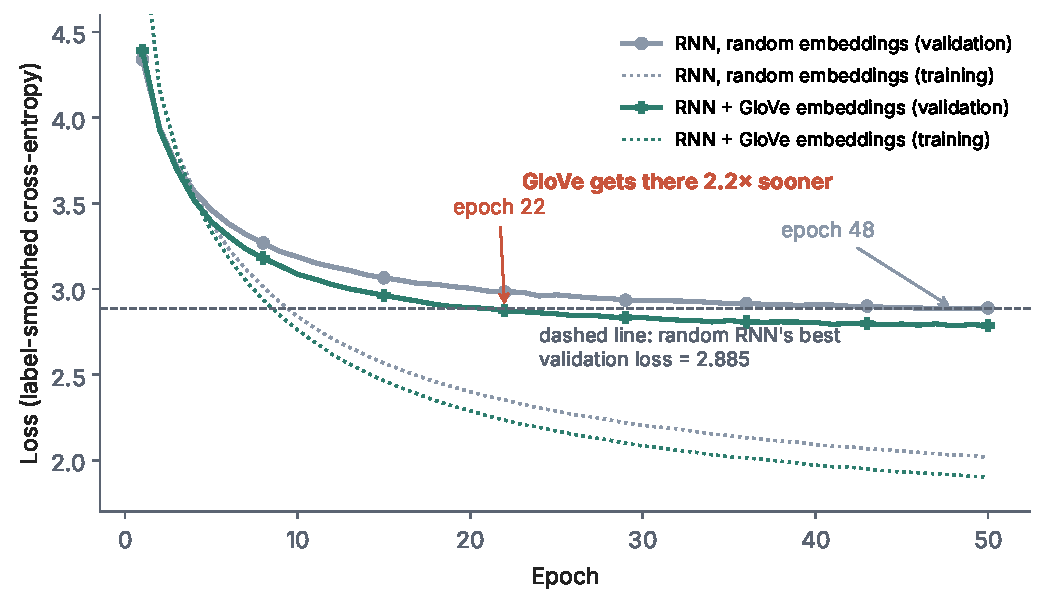
\includegraphics[width=0.85\textwidth]{figures/glove.pdf}
\caption{With \textcolor{cData}{GloVe} the RNN's validation loss falls faster and ends lower.
It crosses the random model's \emph{best} value (dashed line) at epoch 22; the random model only gets there at epoch 48.}
\label{fig:glove}
\end{figure}

Figure~\ref{fig:glove} shows the loss curves for both runs.

\subsection*{Discussion}
\begin{itemize}
\item \textbf{Performance.} GloVe initialisation improves every metric by 2--2.6 points (BLEU +2.6, METEOR +2.6).
  That is almost 60\% of the gap between the plain RNN and the LSTM, with no extra parameters.
  The corpus is small (about 20k sentences), so many English words appear only a few times.
  With random initialisation the model must learn their meaning from those few examples.
  GloVe vectors are trained on 6B tokens and already place related words close together (\emph{italian / french / english}, \emph{happy / glad}).
  The encoder therefore gets meaningful input from the first epoch and generalises better to rare words.
\item \textbf{Training time.} The cost per epoch is identical (3.2 s) because the architecture and parameter count do not change.
  Reading the GloVe file and building the embedding matrix is a one-off cost of a few seconds.
  Convergence is much faster: the GloVe model reaches the random model's \emph{best} validation loss at epoch 22 instead of epoch 48.
  It is also ahead from the first few epochs (epoch 10 val loss: 3.09 vs 3.19). To reach a given quality you need roughly half the training time.
\item \textbf{Limits.} The gains come only from the encoder, because GloVe does not cover Urdu.
  They are bounded by the RNN's fixed-size context vector.
  Some outputs show GloVe's semantic neighbours being confused, e.g.\ \emph{italian} $\rightarrow$ \ur{فرانسیسی} (French).
  Similar words have similar vectors, and the small decoder cannot always tell them apart.
\end{itemize}

\begin{keybox}[Part 4 answer]
Pre-trained GloVe embeddings make the RNN \textbf{better} (about +2.5 on every metric) and \textbf{converge faster}
(the same validation loss in 22 epochs instead of 48), at \textbf{no extra cost per epoch}.
\end{keybox}

% =====================================================================
\section{Conclusion: which model performed best and why?}
% =====================================================================

\begin{keybox}[Answer]
\textbf{The \best{Transformer} is the best model.} It has the highest score on every metric:
BLEU 39.7, ROUGE-L 65.1, METEOR 58.8 and chrF 57.0. It also has the \emph{fewest} parameters (4.9 M). The ranking is

\smallskip
\centering\sffamily\bfseries
\textcolor{cKey}{Transformer} \;>\; \textcolor{cModel}{LSTM $\approx$ BiLSTM} \;>\; \textcolor{cData}{RNN + GloVe} \;>\; \textcolor{cBase}{BiRNN $\approx$ RNN}
\end{keybox}

\textbf{Why:}
\begin{enumerate}[label=\textbf{\arabic*.}]
\item \textbf{Attention replaces the bottleneck.} Every recurrent model squeezes the source sentence into one 256-d vector (Figure~\ref{fig:arch}a).
  The Transformer's multi-head cross-attention lets each Urdu output word look directly at the relevant English words.
  This shows on rare and content words that have to be copied over precisely, e.g.\
  \emph{italian} $\rightarrow$ \ur{اطالوی}, \emph{seldom} $\rightarrow$ \ur{شاذ و نادر}, \emph{your name} $\rightarrow$ \ur{آپ کا نام},
  which the recurrent models replace with frequent words.
  It also shows in ROUGE-2 and chrF, which reward correct word order and correct word forms; there the Transformer leads by 1.7 and 3 points.
\item \textbf{Gating matters for RNNs.} LSTMs beat vanilla RNNs by about 5 BLEU.
  The gates protect the \emph{gradient} (the learning signal) and the memory, so the final encoder state keeps more of the sentence.
  The vanilla RNN's state is dominated by the last few words.
\item \textbf{Bidirectionality helps little here.} BiRNN gains 0.3 BLEU over RNN, and BiLSTM is slightly \emph{worse} than LSTM ($-0.6$).
  Without attention, the decoder only sees the final states, and the sentences are short (about 5 tokens), so the forward state already sees most of the sentence.
  BiLSTM also has 26\% more parameters. It overfits sooner: its best validation loss came at epoch 29 and then rose, while the training loss was the lowest of all models.
\item \textbf{The Transformer had not finished learning.} Its validation loss was still falling at epoch 50, and its best checkpoint is the last one (Figure~\ref{fig:valloss}).
  The other models had plateaued. With more epochs or a learning-rate warm-up schedule, the gap would probably grow.
  Its higher time per epoch (5.8 s vs 3--5 s) comes from the self-attention and cross-attention layers, which do more work per token than a 2-layer RNN on such short sequences.
  It is still under 5 minutes in total on a T4.
\end{enumerate}

Overall, for this small, short-sentence English$\rightarrow$Urdu corpus, \textbf{attention matters more than recurrence type, and recurrence type matters more than bidirectionality.}
Pre-trained embeddings are a cheap way to improve a weak model when data is scarce.

% =====================================================================
\section{Reproducing}
% =====================================================================

\textbf{On Kaggle (GPU).} Push the kernel in the \file{kaggle/} folder. This trains everything from scratch, about 25 minutes on a T4.
\begin{lstlisting}
kaggle kernels push -p kaggle --accelerator NvidiaTeslaT4
\end{lstlisting}

\textbf{Locally.} Put \file{english-corpus.txt}, \file{urdu-corpus.txt} and \file{glove.6B.200d.txt} under \texttt{DATA\_DIR}.
\begin{lstlisting}
DATA_DIR=data python nmt_en_ur.py
\end{lstlisting}
To evaluate the trained weights in \file{results/} without retraining, set \texttt{PRETRAINED\_DIR=results}.
This is how \file{23L-0723_NLP_Assignment-3.ipynb} was executed.

\clearpage
\appendix
\section{All fixed test sentences}
\label{app:examples}

The remaining ten of the 15 fixed test sentences (all 15 are in \file{results/sample_translations.csv}).
\ok\ marks an output identical to the reference, ignoring spacing and final punctuation.

\begin{center}\small
\begin{longtable}{@{}p{2.6cm}>{\raggedleft\arraybackslash}p{10.6cm}c@{}}
\caption{The other ten fixed test sentences. These are harder: only two are ever matched exactly, \textit{he raised his hand} (all six models) and \textit{zain saw everything} (all except RNN + GloVe).}\label{tab:appx}\\
\toprule
\textbf{Model} & \textbf{Urdu output} & \textbf{=\,ref}\\ \midrule \endfirsthead
\toprule \textbf{Model} & \textbf{Urdu output} & \textbf{=\,ref}\\ \midrule \endhead
\bottomrule \endfoot
\rowcolor{cBg}\multicolumn{3}{@{}l@{}}{\textbf{EN:} \textit{whose land is this} \quad \textcolor{cNeutral}{Reference:} \ur{جس کی زمین یہ ہے}}\\*
\textcolor{cBase}{\textbf{RNN}} & \ur{یہ کس کا ہے} & \\*
\textcolor{cBase}{\textbf{BiRNN}} & \ur{یہ کس کا گٹار ہے} & \\*
\textcolor{cModel}{\textbf{LSTM}} & \ur{یہ کس کی پنسل ہے} & \\*
\textcolor{cModel}{\textbf{BiLSTM}} & \ur{یہ کس کی قمیض ہے ؟} & \\*
\textcolor{cKey}{\textbf{Transformer}} & \ur{یہ کس کا مالک ہے} & \\*
\textcolor{cData}{\textbf{RNN + GloVe}} & \ur{یہ کس کا گٹار ہے} & \\
\addlinespace[3pt]
\rowcolor{cBg}\multicolumn{3}{@{}l@{}}{\textbf{EN:} \textit{what is it worth} \quad \textcolor{cNeutral}{Reference:} \ur{اس کی کیا قیمت ہے}}\\*
\textcolor{cBase}{\textbf{RNN}} & \ur{یہ کیا ہے} & \\*
\textcolor{cBase}{\textbf{BiRNN}} & \ur{یہ کیا ہے} & \\*
\textcolor{cModel}{\textbf{LSTM}} & \ur{یہ کیا کام ہے} & \\*
\textcolor{cModel}{\textbf{BiLSTM}} & \ur{یہ کیا ہوا ہے} & \\*
\textcolor{cKey}{\textbf{Transformer}} & \ur{یہ کیا قابل ہے} & \\*
\textcolor{cData}{\textbf{RNN + GloVe}} & \ur{یہ کس چیز ہے} & \\
\addlinespace[3pt]
\rowcolor{cBg}\multicolumn{3}{@{}l@{}}{\textbf{EN:} \textit{does that satisfy you} \quad \textcolor{cNeutral}{Reference:} \ur{کیا یہ آپ کو مطمئن کرتا ہے؟}}\\*
\textcolor{cBase}{\textbf{RNN}} & \ur{کیا یہ آپ کو جانتی ہے ؟} & \\*
\textcolor{cBase}{\textbf{BiRNN}} & \ur{کیا یہ آپ کو تکلیف دیتا ہے} & \\*
\textcolor{cModel}{\textbf{LSTM}} & \ur{کیا اس سے آپ خوفزدہ ہوتے ہیں} & \\*
\textcolor{cModel}{\textbf{BiLSTM}} & \ur{کیا یہ آپ سے محبت کرتا ہے} & \\*
\textcolor{cKey}{\textbf{Transformer}} & \ur{کیا آپ اس سے لطف اندوز ہوتا ہے} & \\*
\textcolor{cData}{\textbf{RNN + GloVe}} & \ur{کیا یہ آپ کی بات کرتا ہے ؟} & \\
\addlinespace[3pt]
\rowcolor{cBg}\multicolumn{3}{@{}l@{}}{\textbf{EN:} \textit{how was your night} \quad \textcolor{cNeutral}{Reference:} \ur{تمہاری رات کیسی گزری}}\\*
\textcolor{cBase}{\textbf{RNN}} & \ur{آپ کا ویک کیسا رہا ؟} & \\*
\textcolor{cBase}{\textbf{BiRNN}} & \ur{آپ کا ویک کیسا تھا ؟} & \\*
\textcolor{cModel}{\textbf{LSTM}} & \ur{آپ کا ویک کیسا تھا} & \\*
\textcolor{cModel}{\textbf{BiLSTM}} & \ur{آپ کا ویک کیسا رہا تھا} & \\*
\textcolor{cKey}{\textbf{Transformer}} & \ur{آپ کا رات کیسا تھا} & \\*
\textcolor{cData}{\textbf{RNN + GloVe}} & \ur{آپ کی رات کیسا تھی ؟} & \\
\addlinespace[3pt]
\rowcolor{cBg}\multicolumn{3}{@{}l@{}}{\textbf{EN:} \textit{zain saw everything} \quad \textcolor{cNeutral}{Reference:} \ur{زین نے سب کچھ دیکھا}}\\*
\textcolor{cBase}{\textbf{RNN}} & \ur{زین نے سب کچھ دیکھا} & \ok\\*
\textcolor{cBase}{\textbf{BiRNN}} & \ur{زین نے سب کچھ دیکھا} & \ok\\*
\textcolor{cModel}{\textbf{LSTM}} & \ur{زین نے سب کچھ دیکھا} & \ok\\*
\textcolor{cModel}{\textbf{BiLSTM}} & \ur{زین نے سب کچھ دیکھا} & \ok\\*
\textcolor{cKey}{\textbf{Transformer}} & \ur{زین نے سب کچھ دیکھا} & \ok\\*
\textcolor{cData}{\textbf{RNN + GloVe}} & \ur{زین نے سب کو دیکھا} & \\
\addlinespace[3pt]
\rowcolor{cBg}\multicolumn{3}{@{}l@{}}{\textbf{EN:} \textit{dont spill the beans} \quad \textcolor{cNeutral}{Reference:} \ur{پھلیاں نہ پھیلائیں}}\\*
\textcolor{cBase}{\textbf{RNN}} & \ur{اس کی مت مت کرو} & \\*
\textcolor{cBase}{\textbf{BiRNN}} & \ur{دروازہ نہ دیں} & \\*
\textcolor{cModel}{\textbf{LSTM}} & \ur{کتے کو مت کھولو} & \\*
\textcolor{cModel}{\textbf{BiLSTM}} & \ur{دروازہ نہ کرو} & \\*
\textcolor{cKey}{\textbf{Transformer}} & \ur{احتیاط مت توڑو} & \\*
\textcolor{cData}{\textbf{RNN + GloVe}} & \ur{باورچی نہ پیو} & \\
\addlinespace[3pt]
\rowcolor{cBg}\multicolumn{3}{@{}l@{}}{\textbf{EN:} \textit{he raised his hand} \quad \textcolor{cNeutral}{Reference:} \ur{اس نے اپنا ہاتھ اٹھایا}}\\*
\textcolor{cBase}{\textbf{RNN}} & \ur{اس نے اپنا ہاتھ اٹھایا} & \ok\\*
\textcolor{cBase}{\textbf{BiRNN}} & \ur{اس نے اپنا ہاتھ اٹھایا} & \ok\\*
\textcolor{cModel}{\textbf{LSTM}} & \ur{اس نے اپنا ہاتھ اٹھایا} & \ok\\*
\textcolor{cModel}{\textbf{BiLSTM}} & \ur{اس نے اپنا ہاتھ اٹھایا} & \ok\\*
\textcolor{cKey}{\textbf{Transformer}} & \ur{اس نے اپنا ہاتھ اٹھایا} & \ok\\*
\textcolor{cData}{\textbf{RNN + GloVe}} & \ur{اس نے اپنا ہاتھ اٹھایا} & \ok\\
\addlinespace[3pt]
\rowcolor{cBg}\multicolumn{3}{@{}l@{}}{\textbf{EN:} \textit{you broke my heart} \quad \textcolor{cNeutral}{Reference:} \ur{تم نے میرا دل توڑا}}\\*
\textcolor{cBase}{\textbf{RNN}} & \ur{آپ نے میرا دل توڑ دیا ۔} & \\*
\textcolor{cBase}{\textbf{BiRNN}} & \ur{تم نے میرا دل توڑ دیا ۔} & \\*
\textcolor{cModel}{\textbf{LSTM}} & \ur{تم نے میرا دل توڑ دیا ۔} & \\*
\textcolor{cModel}{\textbf{BiLSTM}} & \ur{تم نے میرا دل توڑ دیا ۔} & \\*
\textcolor{cKey}{\textbf{Transformer}} & \ur{تم نے میرا دل توڑ دیا ۔} & \\*
\textcolor{cData}{\textbf{RNN + GloVe}} & \ur{تم نے میرا دل توڑ دیا ۔} & \\
\addlinespace[3pt]
\rowcolor{cBg}\multicolumn{3}{@{}l@{}}{\textbf{EN:} \textit{the house was decorated} \quad \textcolor{cNeutral}{Reference:} \ur{گھر سجایا گیا تھا}}\\*
\textcolor{cBase}{\textbf{RNN}} & \ur{گھر بند تھا} & \\*
\textcolor{cBase}{\textbf{BiRNN}} & \ur{گھر بیمار تھا} & \\*
\textcolor{cModel}{\textbf{LSTM}} & \ur{گھر پریتوادت تھا} & \\*
\textcolor{cModel}{\textbf{BiLSTM}} & \ur{گھر خالی تھا} & \\*
\textcolor{cKey}{\textbf{Transformer}} & \ur{گھر پریتوادت تھا} & \\*
\textcolor{cData}{\textbf{RNN + GloVe}} & \ur{گھر گھر تھا} & \\
\addlinespace[3pt]
\rowcolor{cBg}\multicolumn{3}{@{}l@{}}{\textbf{EN:} \textit{i am at your service} \quad \textcolor{cNeutral}{Reference:} \ur{میں آپ کی خدمت میں حاضر ہوں۔}}\\*
\textcolor{cBase}{\textbf{RNN}} & \ur{میں آپ کے قریب ہوں ۔} & \\*
\textcolor{cBase}{\textbf{BiRNN}} & \ur{میں آپ کے بیٹے کے لیے ہوں ۔} & \\*
\textcolor{cModel}{\textbf{LSTM}} & \ur{میں آپ کے اختیار میں ہوں} & \\*
\textcolor{cModel}{\textbf{BiLSTM}} & \ur{میں آپ کی عمر میں ہوں} & \\*
\textcolor{cKey}{\textbf{Transformer}} & \ur{میں آپ کے بالکل پاگل ہوں} & \\*
\textcolor{cData}{\textbf{RNN + GloVe}} & \ur{میں آپ کے ساتھ ہوں ۔} & \\
\end{longtable}
\end{center}

\end{document}
